\begin{savequote}[75mm] 
	Failure is simply the opportunity to begin again, this time more intelligently.
	\qauthor{Henry Ford} 
\end{savequote}

\chapter[(ML)$_\text{2}$ExtraSum: ML based Multi-Lingual Extractive Summarizer]{(ML)$_\text{2}$ExtraSum: Machine Learning based Multi-Lingual Extractive Summarizer}

``Can a system learn to summarize?". 
Many works have been conducted to answer this question applying machine learning (ML) on \ac{ats} problem.
\ac{ml} can be applied as a tuning function \citep{05-yeh-al,10-yatsko-al} where the sentences as scored using many functions, then the system learns how to combine these scores into one. 
It can be used as a decision function \citep{95-kupiec-al,02-osborne} where the system learns to determine if a  sentence belongs to the summary or not. 
Speaking of multilingualism, \ac{ml} based \ac{ats} systems are always bound to the training data's language. 
One idea is to create a model for each language and use a language detector (there exists many open source projects) to select which model to use. 
Even so, the system still partially language-dependent since it cannot process languages outside those it learned to handle. 
Another idea is to train one model using multiple languages. 
This will allow it to extract the shared properties between these languages. 
Of course some recent methods cannot be adapted to do this since they learn to extract their own vocabulary from the training set \citep{15-rush-al,16-nallapati-al,17-ling-rush,17-ren-al}.
Even if the system uses surface features, this proposition makes the system more focused on shared properties and ignores languages particularities.


In this chapter we will present our method (ML)$_\text{2}$ExtraSum which uses surface features related to the document and the sentences and try to score a sentence according to its document. 
We want the system to learn how to score a sentence in multiple ways, then combine these scores into one final score. 
Like \citet{17-ren-al}, the final score must be an estimation of the actual ROUGE-1 measure; thus the system will generate a regression model. 
The system will be trained on multiple languages so it can capture somehow a universal scoring function. 
On the other hand, we do not want it to focus only on shared properties and ignore a language's particularity. 
This is why we train a language clusterer to act like an additional parameter to other scorers. 
Of course this clusterer will not be dependent to the languages it trains on. 
But, it will learns to reduce a given document's features to a more condense representation which can be shared among languages having the same characteristics. 
For instance, if a language \textit{A} tend to have long sentences and two other languages \textit{B} and \textit{C} tend to have shorter ones, the system based on sentences size feature must cluster \textit{B} and \textit{C} closer to each other and far from \textit{A}. 


\section{(ML)$_\text{2}$ExtraSum method overview}

We want to exploit the existing preprocessing tools (LangPi in this case) in order to extract features from text. 
Two types of features are been extracted: document related and sentence related. 
These features can be transformed to be enhanced or to create new features  before being used to score a sentence.
Table~\ref{tab:ml-features} represents the list of surface features used in this method.
\begin{table}[!ht]
	\centering
	\caption{List of features used in ML2ExtraSum.}
	\readtable{ml2extrasum/ml-features.tex}
	\label{tab:ml-features}
\end{table}

Our idea is to express the problem of text summarization as a problem of regression. 
Using some features of a sentence and its document, the system must learn to estimate ROUGE-1 of this sentence based on a reference summary. 
As shown in Figure~\ref{fig:ml2extrasum-archi}, we build some blocks of multi-layer neural networks which we call scorers. 
Each scorer receives one type of features; for instance, there is a scorer which scores a sentence based on its term frequencies and those of its document. 
All these scorers outputs are fed into another scorer to be combined into one final score which is meant to be an estimation of ROUGE-1 score of the sentence in question. 
The system is trained on multiple languages, this is why a block (language clusterer) is reserved to detect the language.
In our case, the language clusterer represent each language as a two dimensional vector which is fed into other scorers so they learn to score based on the language. 

\begin{figure}[ht]
	\centering
	\includegraphics[width=.75\textwidth]{figures/ml2extrasum/archi.pdf} % % %[width=140mm]
	\caption{General architecture of ML2ExtraSum.}
	\label{fig:ml2extrasum-archi}
\end{figure}


Since we want a score between 0 and 1 in the output of every scorer, we use the sigmoid function as an activation function (see Equation \ref{eq:sigmoid}). 
As for the hidden layers, we use \ac{relu} function (see Equation \ref{eq:relu}) to speed up the training phase. 
\begin{equation}
\label{eq:sigmoid}
\sigma(x) = \frac{1}{1 + e^{-x}}
\end{equation}
%
\begin{equation}
\label{eq:relu}
ReLU(x) = \left\lbrace\begin{tabular}{ll}
$ x $ & if $ x > 0 $\\
$ 0 $ & otherwise \\
\end{tabular}\right. 
\end{equation}

We propose four variations of this method, all of them use the same sentence scorer's architecture. 
Its inputs are the outputs of other intermediate scorers as indicated in Equation~\ref{eq:scorer-input}. 
As we said earlier, the language is represented using two values. 
\begin{equation}
\label{eq:scorer-input}
x = \begin{bmatrix}
TF\_score\\ 
Sim\_score\\ 
Pos\_score\\ 
Size\_score\\ 
Lang\_score1\\ 
Lang\_score2\\ 
\end{bmatrix} 
\end{equation}
These inputs are fed into a two fully connected neural hidden layers: the first layer ($ h_1 $) has 50 nodes and the second one ($ h_2 $) has 20 nodes. 
Equation~\ref{eq:scorer-layers} represents the forward propagation equation to predict the sentence score $ \hat{y} $, where $ W_i $ are the weights and $ b_i $ are the biases.
\begin{align}
\label{eq:scorer-layers}
h_1 = ReLU(W_1 x + b_1 ) \nonumber\\
h_2 = ReLU(W_2 h_1 + b_2) \\
\hat{y} = \sigma(W_3 h_2 + b_3) \nonumber
\end{align}
As cost function, we use \ac{mse}  between the predicted score $ \hat{y} $ and ROUGE-1 recall score $ rouge\_1(s_i|S) $ of the sentence $ s_i $ based on a reference summary $ S $. 
\begin{equation}
\label{eq:scorer-mse}
J = MSE = \frac{1}{n} \sum\limits_{i=1}^{n} (\hat{y}_i - rouge\_1(s_i|S))^2
\end{equation}
Where $ n $ is the number of examples in the batch; in our case, it is the number of sentences in the document (the batch is a document). 


\section{Features transformation}

Features can be transformed to ameliorate the scoring function. 
There are two types of features based on their mathematical representations: 
\begin{itemize}
	\item \textbf{Vector representations}: a sentence or a document is represented by a vector of values. 
	The features represented as vectors are: \textit{doc\_tf\_seq}, \textit{doc\_sim\_seq}, \textit{doc\_size\_seq}, \textit{sent\_tf\_seq} and \textit{sent\_sim\_seq}.
	\item \textbf{Scalar representations}: a sentence or a document is represented by one value. 
	The features represented as scalars are: \textit{nbr\_sents}, \textit{sent\_size} and \textit{sent\_pos}.
\end{itemize}
We define three types of transformations: vector to vector, vector to scalar and scalar to scalar.

\subsection{Vector to vector transformations}

To reduce vectors, such as \textit{doc\_tf\_seq}, we use a clipping function which removes low values from the vector. 
We want to keep just the values higher than the arithmetic mean. 
Algorithm~\ref{algo:vec-filter} shows how to filter a given vector from low values.
\begin{algorithm}[!ht]
	\readalgo{ml2extrasum/filter.tex}
	\caption{Filtering vectors by removing values less than the mean.}
	\label{algo:vec-filter}
\end{algorithm}

Sometimes, setting values into a standard range, such as using min-max normalization, can help machine learning. 
Given a vector of values $ \overrightarrow{v} $, the function $ minmax $ that normalizes $ \overrightarrow{v} $ is given in Equation~\ref{eq:vec-norm}. 
\begin{equation}
\label{eq:vec-norm}
minmax(\overrightarrow{v}) = \frac{\overrightarrow{v} - min}{max - min}
\end{equation}
Where $ min $ and $ max $ are given scalars representing the minimum and the maximum boundaries.

\subsection{Vector to scalar transformations}

Sometimes we want to represent a sentence just using one scalar rather than a vector. 
For example, a sentence like its document can both be represented using term frequencies. 
To represent the sentence using a scalar, we want to calculate a portion between its vector and its document's. 
To achieve that, we propose two functions: \textit{S2Dsum} and \textit{S2Dmxmn}.

The first function is called ``sentence to document sum normalization" (\textit{S2Dsum}). 
Given a vector representing a document $ \overrightarrow{D} $ and a vector representing one of its sentences $ \overrightarrow{s} $, the scalar representation of this sentence using S2Dsum is calculated as in Equation~\ref{eq:S2Dsum}.
%
\begin{equation}
\label{eq:S2Dsum}
S2Dsum = \frac{||\overrightarrow{D}|| * sum(\overrightarrow{s})}{||\overrightarrow{s}|| * sum(\overrightarrow{D})}
\end{equation}
Where $ sum $ is a function that sums the values of a vector into one value.


The second function is called ``sentence to document interval normalization" (\textit{S2Dmxmn}). 
Given a vector representing a document $ \overrightarrow{D} $ and a vector representing one of its sentences $ \overrightarrow{s} $, the scalar representation of this sentence using \textit{S2Dsum} is calculated as in Equation~\ref{eq:S2Dmxmn}.
%
\begin{equation}
\label{eq:S2Dmxmn}
S2Dmxmn = \frac{max(\overrightarrow{s}) - min(\overrightarrow{s})}{max(\overrightarrow{D}) * min(\overrightarrow{D})}
\end{equation}
Where $ max $ and $ min $ are functions that lookup the maximum and the minimum values of a vector respectively.


The two previous functions need two vectors to represent one according to the other ($ f: \mathbb{R}^n \times \mathbb{R}^m \rightarrow \mathbb{R} $). 
But, how about a function  that transforms just one vector to a scalar ($ f: \mathbb{R}^n \rightarrow \mathbb{R} $). 
Besides the different average types, we define a function we call ``mean to max normalization" (\textit{meanMax}). 
Given a vector of values $ \overrightarrow{v} $, the function $ meanMax $ that normalizes $ \overrightarrow{v} $ is given in Equation~\ref{eq:meanMax}. 
%
\begin{equation}
\label{eq:meanMax}
meanMax(\overrightarrow{v}) = \frac{mean(\overrightarrow{v})}{max(\overrightarrow{v})}
\end{equation}
Where $ max $ and $ mean $ are functions that lookup the maximum and the mean values of a vector respectively.

\subsection{Scalar to scalar transformations}

The purpose of this transformation is to create more rich features. 
For example, \citet{10-ouyang-al} define four different functions based on word's position in a sentence: Direct proportion (\textit{DP}), Inverse proportion (\textit{IP}), Geometric sequence (\textit{GS}) and Binary function (\textit{BF}). 
Given a scalar $ x $ which is defined from $ 1 $ to $ x_{max} $, we redefine the three first functions as in Equations~\ref{eq:dp}, \ref{eq:ip} and \ref{eq:gs}.
\begin{equation}
\label{eq:dp}
DP(x, x_{max}) = \frac{x_{max} - x}{x_{max}}
\end{equation}
\begin{equation}
\label{eq:ip}
IP(x) = \frac{1}{x}
\end{equation}
\begin{equation}
\label{eq:gs}
GS(x) = (0.5)^{x - 1}
\end{equation}

Sometimes, setting values into a standard range, such as using min-max normalization, can help machine learning. 
Given a scalar $ x $, the function $ minmax $ that normalizes it is given in Equation~\ref{eq:scalar-norm}. 
\begin{equation}
\label{eq:scalar-norm}
minmax(x) = \frac{x - min}{max - min}
\end{equation}
Where $ min $ and $ max $ are given scalars representing the minimum and the maximum boundaries.


Two functions of clipping are used: Maximum clipping (\textit{MxClip}) and Minimum clipping (\textit{MnClip}). 
The two functions are defined in Equations \ref{eq:mxClip} and \ref{eq:mnClip} respectively.
%
\begin{equation}
\label{eq:mxClip}
mxClip(x, x_{max}) = \left\lbrace\begin{tabular}{ll}
$ \frac{x_{max} - x}{x_{max}} $ & if $ x < x_{max} $\\
$ 1 $ & otherwise \\
\end{tabular}\right. 
\end{equation}

\begin{equation}
\label{eq:mnClip}
mnClip(x, x_{min}) = \left\lbrace\begin{tabular}{ll}
$ \frac{x - x_{min}}{x} $ & if $ x > x_{min} $\\
$ 0 $ & otherwise \\
\end{tabular}\right. 
\end{equation}


\section{Method variations}

Our method's implementation varies according to the data transformation step. 
First, we try to consume the features as they are without transformation. 
Then, we filtered all the sequences (TF, sim and sizes) to get more expressive sequences with less storage space. 
The third variation uses normalization so that all the values in the input are between 0 and 1.
The last one is based only on scalar features; we create new features from sequences as well as from scalars.

\subsection{Basic model}

In this model, we use the features as they are in Table~\ref{tab:ml-features} without any transformation. 
Nevertheless, in our experiments we limit the number of sequences to 50 by keeping only the highest values among them. 
These sequences are ordered then fed into \ac{lstm} cells to transform these sequences into one score.
Figure~\ref{fig:ml2extrasum-basic} represents our basic model components (the sentence scorer was explained earlier in Method overview).

\begin{figure}[!ht]
	\centering
	\begin{tabular}{cc}
		\includegraphics[height=.2\textwidth]{figures/ml2extrasum/basic-a.pdf}
		&
		\includegraphics[height=.2\textwidth]{figures/ml2extrasum/basic-b.pdf}
		\\
		(a) Language clusterer & (b) TF or Similarity scorer\\
		\includegraphics[height=.2\textwidth]{figures/ml2extrasum/basic-c.pdf}
		&
		\includegraphics[height=.2\textwidth]{figures/ml2extrasum/basic-d.pdf}
		\\
		(c) Position scorer & (d) Size scorer \\
	\end{tabular}
	
	\caption{Components of the basic model of ML2ExtraSum.}
	\label{fig:ml2extrasum-basic}
\end{figure}

To add language particularity into our scorers, we push into them a 2D language representation (2 scalars). 
This latter is estimated using language clusterer which three \ac{lstm} cells trained on these document features: \textit{doc\_tf\_seq}, \textit{doc\_sim\_seq} and \textit{doc\_size\_seq}.
The logic behind this is that there are languages which tend to repeat words more than others, which have more similar sentences than others or have long sentences.
Figure~\ref{fig:ml2extrasum-basic}(a) represents the architecture of Language clustrer which represents each language as two values.

TF scorer and Similarity scorer both have the same architecture shown in Figure~\ref{fig:ml2extrasum-basic}(b).
The idea is to score a sentence based on two representations: document representation (TF or Sim) and sentence representation (TF or Sim). 
The scoring function is controlled by the two values from Language clusterer. 
This gives them the ability to score a sentence according to the document's language. 
The two sequences doc\_seq and sent\_seq are respectively: \textit{doc\_tf\_seq} and \textit{sent\_tf\_seq} in case of TF scorer, and \textit{doc\_sim\_seq} and \textit{sent\_sim\_seq} in case of Similarity scorer. 
The two sequences are fed into two \ac{lstm} cell with two outputs each, which are concatenated with Language scores.
The four values are the input of two fully connected hidden layers of 50 nodes. 
The output is a perceptron with sigmoid function as it activation function. 

Position scorer is meant to learn how to score a sentence knowing its position, the document's size and the language. 
Figure~\ref{fig:ml2extrasum-basic}(c) represents the architecture of this scorer. 
The input layer is the four scalars: two language scores, \textit{sent\_pos} and \textit{doc\_size}. 
The rest of the architecture is similar to the previous scorer's. 

Size scorer tries to score a sentence using its size based on all document's sizes and its language.
Figure~\ref{fig:ml2extrasum-basic}(c) represents the architecture of this scorer.
We use an \ac{lstm} cell to transform sentences sizes into two scalars. 
These two are concatenated with language scores and \textit{sent\_size} to serve as an input layer. 
The hidden layers and the output one are similar to the previous two scorers. 

\subsection{With filtering}

This one has the same architecture as the previous variant. 
The only difference is filtering the sequences: \textit{doc\_tf\_seq}, \textit{doc\_sim\_seq}, \textit{doc\_size\_seq}, \textit{sent\_tf\_seq} and \textit{sent\_sim\_seq} before feeding them into the system. 
For each sequence, the system uses just the values higher than the mean. 
This will reduce the working space and will help the system focusing on the most important values.

\subsection{With normalization and filtering}

Normalizing the values helps the system converging faster. 
The architecture stays the same as the basic one; the only difference is in Features transformation step. 
This is a list of features and the transformation functions applied to them:
\begin{itemize}
	\item We apply a min-max normalization then a filtering function on: \textit{doc\_tf\_seq}, \textit{doc\_size\_seq} and \textit{sent\_tf\_seq}. 
	The min and max values are the calculated from the document. 
	For example, to normalize \textit{doc\_tf\_seq} or \textit{sent\_tf\_seq} both take the maximum TF in the document as max and the minimum tf in the document as min.
	\item We apply a filtering function on: \textit{doc\_sim\_seq} and \textit{sent\_sim\_seq}. 
	Their values are known between 0 and 1, therefore no need to normalize.
	\item The scalar \textit{sent\_size} is normalized, where \textit{max} (\textit{min}) is the maximum (minimum) size of sentences in the document.
\end{itemize}
The scalar \textit{doc\_size} is not normalized since the training batch is a document. 
Also, \textit{sent\_pos} is not normalized since it is used with \textit{doc\_size}. 


\subsection{With scalar features}

In this version, we want to use just scalar features (no sequences) and create new features as well. 
Then, each type of features is fed into its related scorer as an input layer. 
The intermediate scorers, in this version, have all just one layer of 50 perceptrons. 
They have one output, expect of language clusterer which has two. 
Figure~\ref{fig:ml2extrasum-pure} shows the new created features using the transformation functions we presented earlier.
The new size features are based on min and max clipping, where the minimum and maximum limits are calculated from document's sizes by weighting the mean and the max sizes. 
The weights we used in our system are: $ \alpha 1 = 0.7 $, $ \alpha 2 = 1.3 $, $ \beta 1 = 0.3 $ and $ \beta 2 = 0.7 $.
%
\begin{figure}[!ht]
	\centering
	\includegraphics[width=\textwidth]{figures/ml2extrasum/pure.pdf} % % %[width=140mm]
	\caption{New scalar features created using transformation of the old ones.}
	\label{fig:ml2extrasum-pure}
\end{figure}


\section{Experiments}

%\subsection{Metrics}

In our evaluation, we use two metrics of ROUGE: ROUGE-1 and ROUGE-2, which are used in most automatic text summarization workshops.
For that matter, we use LangPi implementation of ROUGE (see Appendix A).
As for the baseline, we use our TCC method described in Chapter~\ref{chap:tcc} and implemented in AllSummarizer system (see Appendix A). 

\subsection{Corpus preparation}

In our experiments we use MultiLing 2015 Multi-lingual Single-document Summarization (MSS) corpora which is designed for multilingual summarization. 
The corpus has been pre-processed using LangPi to extract some statistics. 
The new corpus's structure is represented in Figure~\ref{fig:ml2extrasum-corpus}.
The corpus can be downloaded from the first release of ML2ExtraSum project\footnote{ML2ExtraSum corpus: \url{https://github.com/kariminf/ML2ExtraSum/releases/tag/1.0.0} [25 August 2019]}.

\begin{figure}[!ht]
	\centering
	\includegraphics[width=.3\textwidth]{figures/ml2extrasum/corpus.pdf} % % %[width=140mm]
	\caption{ML2ExtraSum corpus structure.}
	\label{fig:ml2extrasum-corpus}
\end{figure}

The corpus contains 40 folders representing languages used in MultiLing'15. 
Each folder contains a json file named ``\textbf{lang.json}", which affords the following information: 
\begin{itemize}
	\item \textit{maxSentTFLength} and \textit{maxSentSimLength} : The size of the longest sentence TF and similarity vectors in all sentences of the language.
	\item \textit{maxDocTFLength}, \textit{maxDocSimLength} and \textit{maxDocSizesLength}: The size of the longest document TF, similarity and sizes vectors in all documents of the language.
\end{itemize}
Each language contains 30 documents represented by folders which contains the following json files:
\begin{itemize}
	\item \textbf{docInfo.json}: it affords statistics about the document:
	\begin{itemize}
		\item \textit{size}: the number of sentences in the document.
		\item \textit{sizes}: a vector representing the sizes of each sentence in term of words.
		\item \textit{sims}: a vector representing cosine similarities between each sentence and the whole document.
		\item \textit{freqs}: a vector representing words frequencies.
		\item \textit{maxSentSimLength}: the size of the longest similarity vector.
		\item \textit{maxSentTFLength}: the size of the longest TF vector.
	\end{itemize}

    \item \textbf{sentLen.json}: it affords statistics about sentences lengths (sizes). The key is the sentence position and the value is the sentence size (number of words).
    
    \item \textbf{sentRouge1.json}: it affords statistics about sentences ROUGE-1 scores. The key is the sentence position and the value is the sentence ROUGE-1 score.
    
    \item \textbf{sents.json}: It affords sentences. The key is the sentence position and the value is the sentence.
    
    \item \textbf{sentSim.json}: it affords statistics about sentences similarity scores. The key is the sentence position and the value is a vector of non zero similarities (there is no order).
    
    \item \textbf{sentTF.json}: it affords statistics about sentences TF scores. The key is the sentence position and the value is a vector of its words frequencies in the document.
    
\end{itemize}

\subsection{Experiments setup}

ML2ExtraSum\footnote{ML2ExtraSum: \url{https://github.com/kariminf/ML2ExtraSum} [25 August 2019]} system is implemented using Python and it has been open-sourced on Github under Apache 2.0 license. 
It requires \textbf{json} library to read the statistics we generated earlier, \textbf{matplotlib} to plot languages scores, \textbf{numpy} to handle arrays and matrices, and \textbf{tensorflow} to build neural networks. 

Algorithm~\ref{algo:training} demonstrates the steps followed to train our models. 
As you can notice, we used each document as a batch rather than a language or the whole training set. 
This is because loading all the dataset at once will overload the memory. 
So, the execution time has been sacrificed by reading the documents from disk over and over again. 
\begin{algorithm}[!ht]
	\readalgo{ml2extrasum/training.tex}
	\caption{Training steps used on ML2ExtraSum system.}
	\label{algo:training}
\end{algorithm}


After training our models, they are used to score the sentences of the testing dataset. 
Algorithm~\ref{algo:testing} shows the steps followed to test a given model (we generated 4 models). 
To extract a summary based on sentences scores, we used two extraction methods: the plain one based on the scores order and the one proposed in \citep{15-aries-al} based on sentences similarities. 
We do not just use the final score, but also we use intermediate scores of each block. 
We extracted summaries using AllSummarizer\_TCC \citep{13-aries-al,15-aries-al} as a baseline. 
Also, we extracted summaries using the actual ROUGE-1 scores to see what our system should do if it estimates ROUGE-1 correctly. 
\begin{algorithm}[!ht]
	\readalgo{ml2extrasum/testing.tex}
	\caption{Testing steps used on ML2ExtraSum system.}
	\label{algo:testing}
\end{algorithm}


\subsection{Results}

We tested 40 languages, 4 models and 2 extraction methods. 
When it comes to plotting the results or even showing them in a table, it renders them to be unreadable.  
This is why we chose just 8 languages as an example:
\begin{itemize}
	\item Two Semitic languages: Arabic (ar) and Hebrew (he).
	\item Two Germanic languages: English (en) and German (de).
	\item Two Romance languages: French (fr) and Spanish (es).
	\item Two separate Asiatic languages: Japanese (ja) and Chinese (zh). Although they do not belong to the same language family, they share almost the same writing system which is Chinese originally. 
\end{itemize}

Also, for the sake of shortness, lets call our models as follows:
\begin{itemize}
	\item \textit{basic}: The basic model with the initial features.
	\item \textit{filter}: The model where sequences are filtered using the mean value.
	\item \textit{norm}: The model where the features are normalized, then the sequences are filtered. 
	\item \textit{pure}: The model with only scalar features created from the initial ones.
\end{itemize}

\subsubsection{Summarization task results}


To compare ML2ExtraSum's performance, we used AllSummarizer\_TCC as a baseline system. 
This latter uses an extractive method based on surface statistical features: grams' frequency, sentence position and size. 
Also, to determine what the system is supposed to perform if it estimates a sentence's ROUGE-1 perfectly, we used the actual ROUGE-1 scores for generation. 
As shown in Table~\ref{tab:lang-meth-compare}, the system is not doing as well as what is is supposed to do for all its variants. 
The variants cannot even beat the baseline (AllSummarizer\_TCC) in all the 8 languages.  
The values in bold are the highest among ML2ExtraSum's variants. 
It is clear that \textit{pure} variant is doing better compared to other variants. 

\begin{table}[!ht]
	\centering
	\small
	\caption{ROUGE-1 recall scores of summaries generated using ML2ExtraSum compared to AllSummarizer\_TCC and real ROUGE-1 generation.}
	\readtable{ml2extrasum/lang-meth-compare.tex}
	\label{tab:lang-meth-compare}
\end{table}


We want to test how well the intermediate scorers are doing: TF scorer (tf), Similarity scorer (sim), Position scorer and Size scorer (size). 
Also, we tried the sum of these scores (sums) as a sentence importance score. 
Since \textit{pure} model is the highest scored among the others, we use it to compare between the final sentence score (sent) and the intermediate ones as shown in Table~\ref{tab:pure-inter-compare}.
In bold, the values that exceed the sentence summaries ROUGE-1 recall.
As shown in the table, most summaries using similarity scorer are better than those using final sentence score in term of ROUGE-1 recall. 
This implies that there are some features which decrease system's performance when being used. 
Perhaps it is better to train a features selector which selects which feature to use by the system.

\begin{table}[ht]
	\centering
	\small
	\caption{ROUGE-1 recall scores of summaries generated using ML2ExtraSum \textit{pure} model's intermediate scores.}
	\readtable{ml2extrasum/pure-inter-compare.tex}
	\label{tab:pure-inter-compare}
\end{table}

To compare ML2ExtraSum with AllSummarizer\_TCC, we used similarity based extraction method used by this latter. 
For all the models and 40 languages, the only time ML2ExtraSum beats AllSummarizer\_TCC based on the sentence estimated score is using \textit{pure} model with Afrikaans (af) language. 
Based on TF scorer, it beats it using filter model in 2 languages (eu, th) and using pure model in 7 languages (eu, he, id, it, ja, nl, th). 
Based on Similarity scorer, it beats it only using pure model in 7 languages (en, eu, it, ja, ka, no, th). 
Based on Pos scorer, it beats it only using pure model in 3 languages (af, fa, ja). 
It is clearly that trying to train a system based on some predefined features do no good compared to a data-free method (no training) using the same features, at least using the proposed architecture.  


\subsubsection{Language clustering results}

In this section, we want to evaluate our models based on their capacity to differentiate between languages based on three criteria: their higher term frequencies, their higher sentences similarities and their higher sentences sizes (in term of words).
Using each model, for each language (8), we plotted a graph of its 30 documents' language scores afforded by language clusterer (see Figure~\ref{fig:lang-scores}). 

\afterpage{
\begin{landscape}
\begin{figure}[!ht]
	\centering
	\begin{tabular}{cc}
		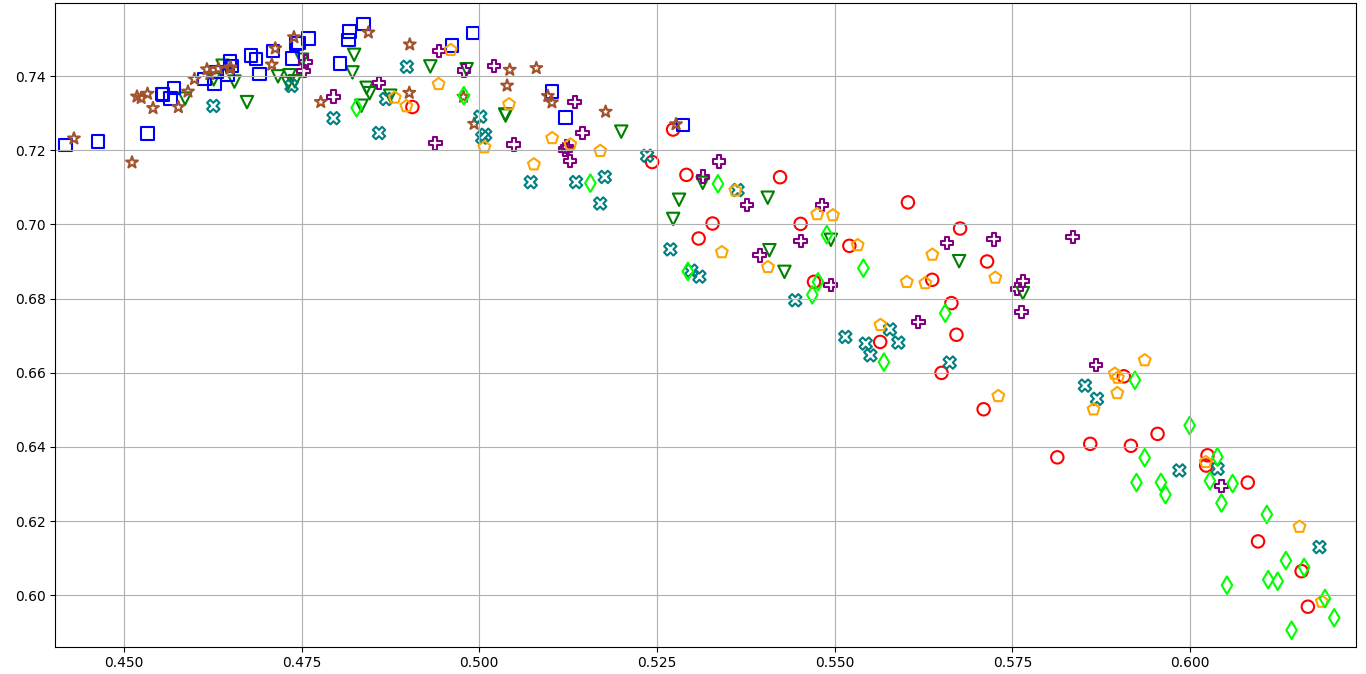
\includegraphics[height=0.35\textheight]{figures/ml2extrasum/lang-basic.png} &
		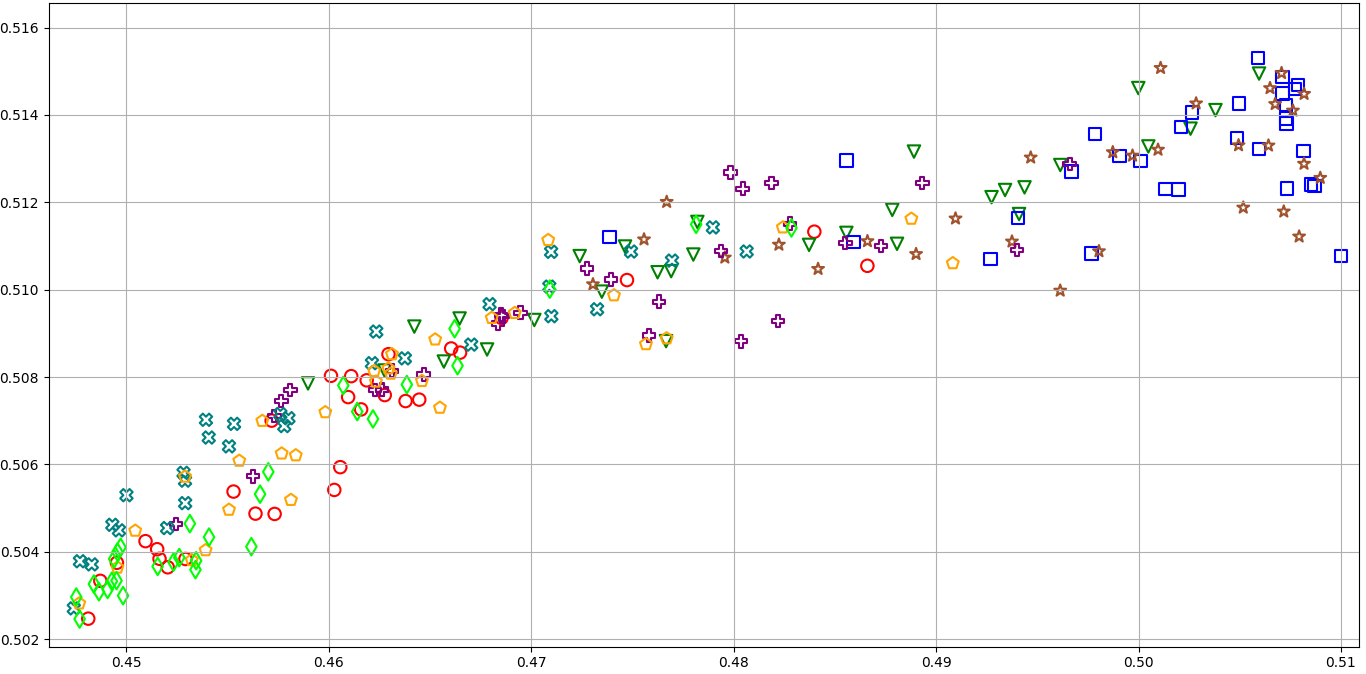
\includegraphics[height=0.35\textheight]{figures/ml2extrasum/lang-filter.png} \\
		(a) using \textit{basic} model & (b) using \textit{filter} model \\
		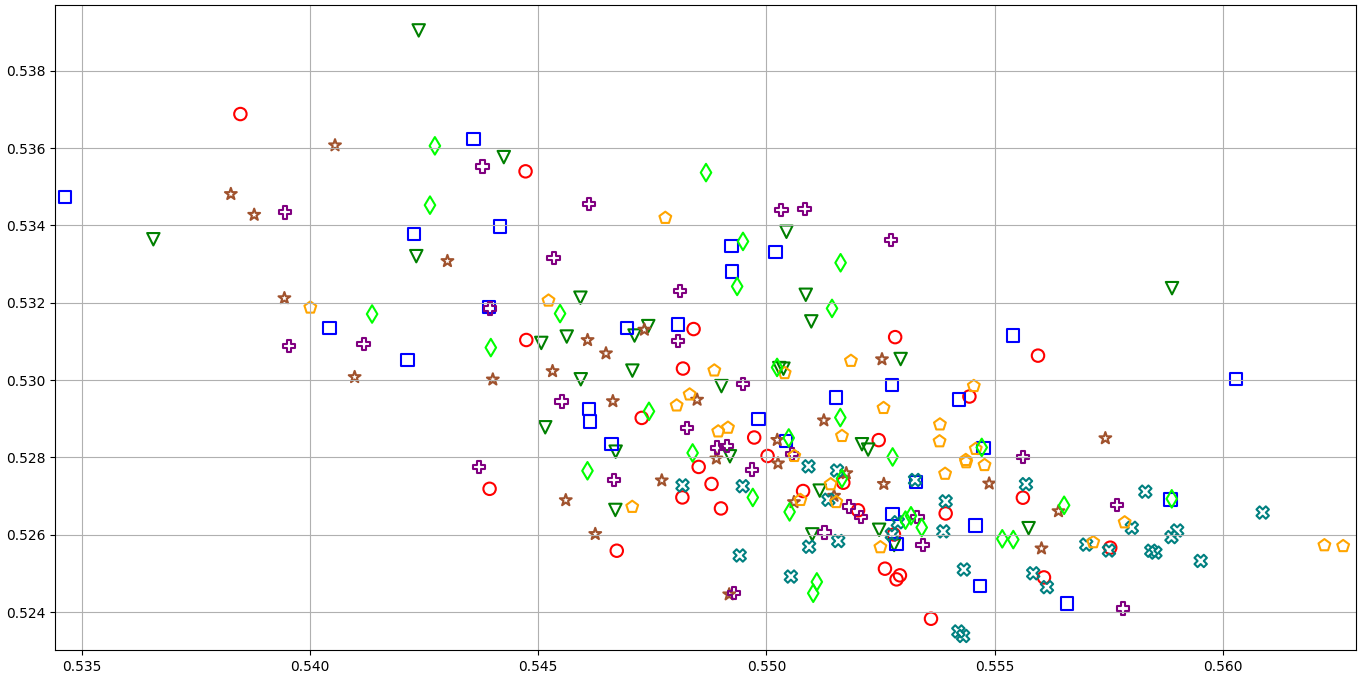
\includegraphics[height=0.35\textheight]{figures/ml2extrasum/lang-norm.png} &
		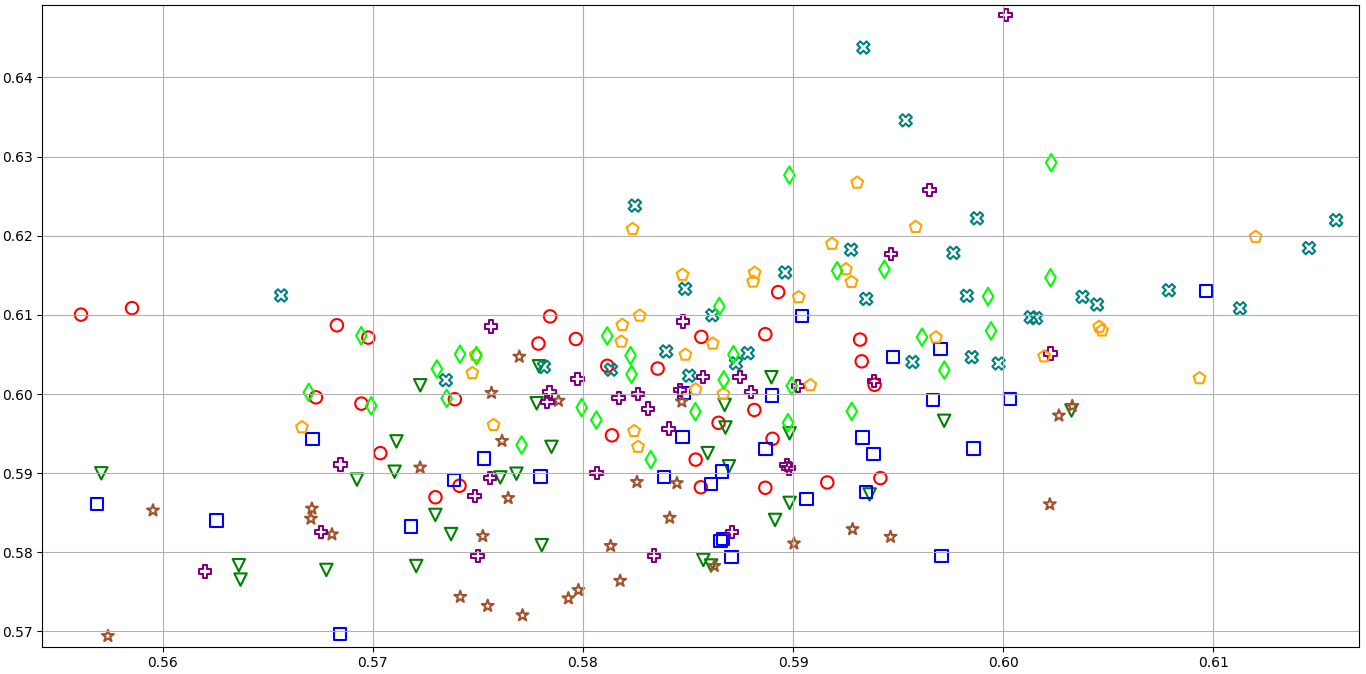
\includegraphics[height=0.35\textheight]{figures/ml2extrasum/lang-pure.png} \\
		(c) using \textit{norm} model & (d) using \textit{pure} model  \\
		\multicolumn{2}{c}{
\includegraphics{figures/ml2extrasum/lang-legend.png}}
	\end{tabular}
	
	\caption{ML2ExtraSum Language scores for 8 languages based on testing corpus using the 4 models.}
	\label{fig:lang-scores}
\end{figure}
\end{landscape}
}

The \textit{basic} model did a good job on clustering the languages, though the interval is too small which is from (0.44, 0.59) to (0.62, 0.75). 
We can see that the two Germanic languages are the most distinct among the others. 
All their documents are situated between (0.41,0.72) and (0.53, 0.76) which is a narrow space compared to others. 
This can tell us that English and Germany may share the same characteristics in term of TF, similarities and sizes. 
Also, it shows that the system learned this information perfectly.
The other languages' documents are not as separable as those of the previous ones. 
Nevertheless, we notice that most documents of each language are situated in the same place: Hebrew to the left; Arabic, French, Japanese and Spanish dispersed in the center; and Chinese which is mostly to the right. 

Filtering the sequences, as shown in Figure~\ref{fig:lang-scores}(b), appears to enhance language clustering. 
It seems that documents of the same language are closer to each other compared to the \textit{basic} model.
This allows us to hypothesize that clustering a document language gives the importance to higher values in our three sequence features.
Nevertheless, the scores' range is too narrow; going from (0.447, 0.502) to (0.51, 0.516). 
Another observation is that the scores using both \textit{basic} and \textit{filter} models are arranged in a linear form rather than spreading over the plane.
This can tell us that using just one dimension is enough to represent the different languages based on these two models. 


Unlike the past two models, normalizing the input values allows the system to represent languages in a two dimensional way as shown in Figure~\ref{fig:lang-scores}(c). 
Except for Spanish and Japanese, it seems that all documents of each language are scattered all around the plane. 
A good clustering would separate each language apart.  
Anyways, just three features is not sufficient to separate as much languages since many languages share the same characteristics. 


Likewise, creating new scalar features before being fed into the system does not do it any favor as shown in Figure~\ref{fig:lang-scores}(d).
The system learns to represent the language in a two dimensional way.
However, these languages are not really separable since most of their documents are swarming into the same place. 
That being said, a given language's documents seem to deviate a little from others of a different language. 
It is not enough to separate them apart, but still promising. 
Maybe, creating more features will help enhancing this task. 


\section{Discussion}

% method description 
We presented an extractive method for multi-lingual text summarization based on machine learning. 
In this method, we use surface statistical features which are weakly dependent on language.
These features can be related to the sentence to be scored or its document; they include: terms frequencies, sentences sizes, sentences similarities, document size and sentences positions. 
The sentence is scored using many scorers: TF scorer, Similarity scorer, Position scorer and Size scorer. 
These scorers use their adequate features beside a score afforded by a language clusterer so they do not score all languages the same. 
The scores afforded by these scorers beside the language clusters are combined using another scorer to afford the final score. 
In our case, this score must be ROUGE-1 score of the sentence in question compared to a reference summary. 
So in summary, the method wants to learn how to estimate ROUGE-1 score of a sentence using some surface features. 
The training uses the actual ROUGE-1 scores; but when trained, the system must estimate what the score will be without referring to any existing summary.


The method was implemented as a system called ``ML2ExtraSum" using neural networks resulting in 4 variants. 
The first variant (\textit{basic}) uses the statistical features as they are without transformation. 
The sequences are fed into an LSTM cell to learn how to reduce their dimension into one or two scalars. 
The second variant (\textit{filter}) is similar to the first, but it filters the sequences by deleting the values under the mean. 
Our assumption is that this will allow the system to focus only on the important values. 
The third variant (\textit{norm}) is similar to the first, but it normalizes the features and filters the sequences before feeding them into the neural network. 
This is done in hope that the normalization will improve the system's performance. 
The fourth variant (\textit{pure}) uses pure scalars as input. 
We generated some new features which are scores in some sort and fed them into the system so it will learn how to combine them into intermediate scores, then a final one. 

To test our system, we used AllSummarizer\_TCC \citep{13-aries-al,15-aries-al}, which does not use machine learning at all, as a baseline system. 
Unfortunately, ML2ExtraSum had no chance against AllSummarizer\_TCC in any of its variants. 
This tells us that our \ac{ml} based architecture maybe needs more than some surface features to reach its full potential. 
Another assumption is that \ac{ml} is not as fit to score the pertinence of a sentence in a multi-lingual context as a traditionally encoded solution based on observation does. 
At least, not in the way our architecture is proposed. 
We must, also, take in consideration that the training batch was a document. 
So, if the whole dataset was used as a batch, result might be different.
Letting the system extracting the features by itself such as using word embedding is interesting, but it will require sacrificing the multi-lingual aspect of the system. 
Moreover, it will consume a lot of data to construct a valid vocabulary. 

%As future directions, we will investigate how adding more features can affect the system's performance.
%Nowadays, there are tools that afford some deep language features for multiple languages, such as BabelNet\footnote{BabelNet website: \url{https://babelnet.org/} [27 August 2019]} \cite{12-naigli-ponzetto}.
%Also, generating more new features may help the system as shown by \textit{pure} model in our experiments. 
%On the bright side, the system shows promising results when it comes to clustering languages based on summarization.
%Same as scoring, the task of clustering  still has to be improved so it can separate languages and represent them in a larger range.





